% ==================================================================
%  Group-seminar talk on the manuscript
%  "Zero-point flux fluctuations switch a quantum-dot Josephson loop from 0 to pi"
%  Build:  cd talk && pdflatex talk.tex (twice)
%  Figures: ../figs/* (manuscript figures) and figs/* (make_talk_figs.py, teaching figures)
% ==================================================================
\documentclass[aspectratio=169,9pt]{beamer}
\usetheme[progressbar=frametitle,numbering=fraction,block=fill]{metropolis}
\usepackage[T1]{fontenc}
\usepackage{lmodern}
\usepackage{amsmath,amssymb,bm,mathtools}
\usepackage{physics}
\usepackage{booktabs,array}
\usepackage{tikz}
\usetikzlibrary{arrows.meta,decorations.pathmorphing,positioning,calc,shapes.geometric}
\usepackage[american,siunitx]{circuitikz}
\usepackage[most]{tcolorbox}
\usepackage{appendixnumberbeamer}

% ---------------------------------------------------------------- colours
\definecolor{ink}{HTML}{1F2A44}
\definecolor{accent}{HTML}{2A6FDB}
\definecolor{warm}{HTML}{E8692B}
\definecolor{good}{HTML}{1AA37A}
\definecolor{purp}{HTML}{5B3FA8}
\definecolor{paper}{HTML}{FAFAF7}
\setbeamercolor{normal text}{fg=ink,bg=paper}
\setbeamercolor{alerted text}{fg=warm}
\setbeamercolor{frametitle}{bg=ink,fg=white}
\setbeamercolor{progress bar}{fg=warm,bg=ink!30}
\setbeamercolor{example text}{fg=good}
\setbeamercolor{block title}{bg=accent!15,fg=ink}
\setbeamercolor{block body}{bg=accent!5}
\setbeamercolor{block title alerted}{bg=warm!20,fg=ink}
\setbeamercolor{block body alerted}{bg=warm!6}
\setbeamercolor{block title example}{bg=good!18,fg=ink}
\setbeamercolor{block body example}{bg=good!6}
\setbeamertemplate{itemize items}{\color{accent}$\blacktriangleright$}

\newtcolorbox{keybox}[1][]{enhanced,colback=accent!6,colframe=accent,boxrule=0.8pt,arc=2mm,
  left=2mm,right=2mm,top=1mm,bottom=1mm,before upper=\raggedright,#1}
\newtcolorbox{warnbox}[1][]{enhanced,colback=warm!7,colframe=warm,boxrule=0.8pt,arc=2mm,
  left=2mm,right=2mm,top=1mm,bottom=1mm,before upper=\raggedright,#1}
\newtcolorbox{calcbox}[1][]{enhanced,colback=white,colframe=ink!40,boxrule=0.5pt,arc=1mm,
  left=2mm,right=2mm,top=0.5mm,bottom=0.5mm,before upper=\raggedright,fonttitle=\small\bfseries,coltitle=ink,colbacktitle=ink!8,#1}

\newcommand{\hw}{\hbar\omega}
\newcommand{\Hring}{H_{\rm ring}}
\newcommand{\pcl}{\varphi_{\rm cl}}
\newcommand{\cw}{\circlearrowright}
\newcommand{\ccw}{\circlearrowleft}
\newcommand{\hl}[1]{\textcolor{accent}{#1}}
\renewcommand{\cite}[1]{{\scriptsize\textcolor{ink!60}{[#1]}}}
\newcommand{\figsrc}[1]{\par\vspace{-1mm}{\tiny\hfill\textcolor{ink!50}{#1}}}

\graphicspath{{../figs/}{figs/}}

\title{Zero-point flux fluctuations switch a quantum-dot Josephson loop from $0$ to $\pi$}
\subtitle{An exact electron--photon solution of a $\pi$ loop sharing its inductance with a cavity mode}
\author{Group seminar}
\date{}

\begin{document}

% ==================================================================
\begin{frame}[plain]
  \titlepage
\end{frame}

% ------------------------------------------------------------------
\begin{frame}{The story in one slide}
  \begin{columns}[c]
    \column{0.42\textwidth}
    \centering
    \begin{circuitikz}[scale=0.85,transform shape]
      \draw[blue!70!black,line width=1.1pt] (0,0) to[L,l=$L$,color=blue!70!black] (0,2.6);
      \draw[blue!70!black] (0,2.6) -- (-1.3,2.6) to[C,l_=$C$,color=blue!70!black] (-1.3,0) -- (0,0);
      \draw[line width=2pt] (0,2.6) -- (3,2.6) -- (3,1.65);
      \draw[line width=2pt] (3,0.95) -- (3,0) -- (0,0);
      \draw[thick,fill=white] (2.7,0.95) rectangle (3.3,1.65);
      \fill[warm] (3,1.3) circle (0.09);
      \node[right] at (3.35,1.55) {$\pi$};
      \node[right,warm] at (3.35,1.05) {$U$};
      \draw[-{Stealth[length=2.5mm]},thick,ink!70] (1.95,1.85) arc (60:120:0.9);
      \draw[-{Stealth[length=2.5mm]},thick,ink!70] (1.05,0.75) arc (240:300:0.9);
      \node at (1.5,1.3) {$\pm I$};
      \node[blue!70!black] at (-0.6,3.0) {$\hw\,a^\dagger a$};
    \end{circuitikz}
    \par\small A BCS ring closed by an \alert{interacting quantum dot}, threaded by the quantized flux of one $LC$ mode.
    Solved \emph{exactly} (DMRG on electrons $\otimes$ photon).
    \column{0.58\textwidth}
    \begin{enumerate}\small
      \item \textbf{The vacuum of the mode controls the junction.} Its zero-point flux moves the singlet--doublet
            ($0$--$\pi$) boundary: at $Z\simeq2\,$k$\Omega$ ($g\simeq0.5$) a $0$ junction becomes a $\pi$ junction.
            Adiabatic mechanism (curvatures of $E_s(\varphi)$) $\to$ Franck--Condon mechanism ($t_J\to t_Je^{-g^2/2}$).
      \item \textbf{Full-DMRG phase diagram in $(U,g)$.} For $U>U_c$, $g>g_c(U)$ the mode condenses
            ($\langle a\rangle\neq0$ = a persistent current). This is the classical screening instability $\beta>1$ of a
            $\pi$ loop; the exact ground state is a \alert{cat} of the two current directions, and zero-point motion pushes
            the threshold above $\beta=1$.
      \item \textbf{The product-state mean field orders where the exact solution does not}: for $E_J\lesssim3\hw$ and at
            $U\simeq U_c$, where a static moment replaces the Kramers doublet.
    \end{enumerate}
  \end{columns}
\end{frame}

% ------------------------------------------------------------------
\begin{frame}{Outline}
  \setbeamertemplate{section in toc}[sections numbered]
  \tableofcontents
\end{frame}

% ==================================================================
\section{Background and what is new}

\begin{frame}{$\pi$ loops, photon condensation, and the no-go theorem}
  \begin{columns}[T]
    \column{0.5\textwidth}
    \textbf{Known since 1977:} a loop closed by a $\pi$ junction carries a spontaneous current when
    $L>\Phi_0/2\pi I_c$ \cite{Bulaevskii--Kuzii--Sobyanin 1977; Tsuei--Kirtley 2000; Bauer 2004}; with a small $C$
    the two directions form a flux qubit without external field \cite{Ioffe 1999; Kawabata 2006; Feofanov 2010}.
    \vspace{1mm}
    \textbf{Cavity QED version:} a mode coupling through its \emph{flux} evades the no-go theorem for superradiance
    and condenses a static field $\langle a\rangle\neq0$ \cite{Nataf--Ciuti 2010; Bamba 2016; Andolina 2020; Mercurio 2024}
    -- the condition is the magnetostatic instability of the matter.
    \column{0.5\textwidth}
    \begin{keybox}[title={What was missing}]
      \small In all of these the junction is a \emph{fixed} function $E(\varphi)$, or electrons and mode are decoupled
      in a product state \cite{Varrica 2026}.
    \end{keybox}
    \begin{keybox}[title={This work}]
      \small A \alert{quantum-dot} junction is not a fixed $E(\varphi)$: it is $\pi$ only in its doublet state, and
      whether it is $0$ or $\pi$ is decided by $U$, $\Gamma$, $\Delta$ on a scale of a few GHz -- comparable to $\hw$.\\[1mm]
      $\Rightarrow$ treat electrons and quantized flux on the same footing and solve \emph{exactly} by DMRG
      \cite{cf. Passetti 2023; Bacciconi 2023}.
    \end{keybox}
  \end{columns}
\end{frame}

% ------------------------------------------------------------------
\begin{frame}{Warm-up: 0 and $\pi$ Josephson junctions}
  \begin{columns}[c]
    \column{0.5\textwidth}
    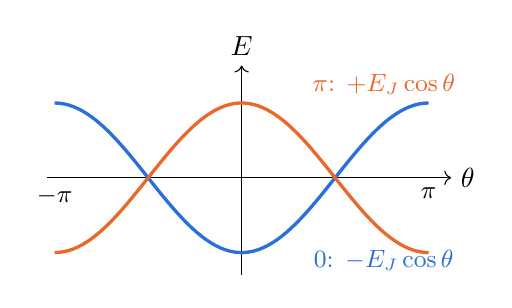
\begin{tikzpicture}[scale=0.95]
      \draw[->] (-2.6,0) -- (2.8,0) node[right] {$\theta$};
      \draw[->] (0,-1.3) -- (0,1.5) node[above] {$E$};
      \draw[accent,very thick,domain=-2.5:2.5,samples=80] plot (\x,{-cos(deg(\x*1.257))});
      \draw[warm,very thick,domain=-2.5:2.5,samples=80] plot (\x,{cos(deg(\x*1.257))});
      \node[accent] at (1.9,-1.1) {\small $0$: $-E_J\cos\theta$};
      \node[warm] at (1.9,1.25) {\small $\pi$: $+E_J\cos\theta$};
      \foreach \x/\l in {-2.5/-\pi,2.5/\pi} \node[below] at (\x,0) {\small$\l$};
    \end{tikzpicture}
    \par\small $\theta$ = gauge-invariant Cooper-pair phase difference.
    \column{0.5\textwidth}
    \begin{itemize}\small
      \item \textbf{0 junction:} minimum at $\theta=0$, $E''>0$: an \emph{inductance} $L_J=(\Phi_0/2\pi)^2/E_J$, diamagnetic.
      \item \textbf{$\pi$ junction:} minimum at $\theta=\pi$; at $\theta=0$ a \emph{maximum}: a \alert{negative inductance},
            paramagnetic.
      \item Realizations: SFS, $d$-wave corners, and \alert{quantum dots with a local moment} (this talk).
    \end{itemize}
    \begin{calcbox}[title={Classical $\pi$ rf-SQUID}]
      \small $U(\theta)=\frac{E_L}{2}\theta^2+E_J\cos\theta$, \ $E_L=\frac{(\Phi_0/2\pi)^2}{L}$.\\
      $U''(0)=E_L-E_J<0$ iff $\beta\equiv\frac{E_J}{E_L}=\frac{2\pi LI_c}{\Phi_0}>1$.
    \end{calcbox}
  \end{columns}
\end{frame}

% ------------------------------------------------------------------
\begin{frame}{Why a quantum dot with a local moment is a $\pi$ junction}
  \begin{columns}[T]
    \column{0.52\textwidth}
    \small Anderson impurity between BCS leads. Two competing ground states of the ring:
    \begin{itemize}\small
      \item \textbf{singlet} (even fermion parity): the dot electron is screened/paired; a $0$ junction, $E_2<0$;
      \item \textbf{doublet} (odd parity, Kramers pair): a Cooper pair crosses by fourth-order cotunnelling, one
            electron at a time, and arrives with its spins in \alert{reversed order}:
            $c^\dagger_\downarrow c^\dagger_\uparrow=-c^\dagger_\uparrow c^\dagger_\downarrow$ $\Rightarrow$ $E_J\to-E_J$, a $\pi$ junction, $E_2>0$.
    \end{itemize}
    \small \cite{Glazman--Matveev 1989; Spivak--Kivelson 1991; Vecino 2003; Karrasch 2008}; seen in nanowire and CNT dots
    \cite{van Dam 2006; Cleuziou 2006; Delagrange 2015}; read out via a transmon/resonator \cite{Bargerbos 2022; Hays 2021}.
    \column{0.46\textwidth}
    \centering
    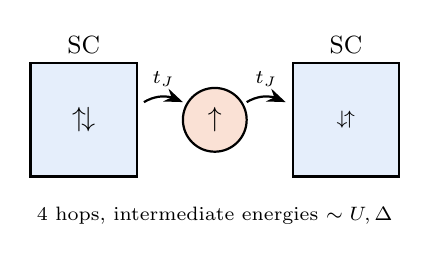
\begin{tikzpicture}[scale=0.9]
      \draw[thick,fill=accent!12] (-2.6,-0.8) rectangle (-1.1,0.8); \node at (-1.85,1.05) {\small SC};
      \draw[thick,fill=accent!12] (1.1,-0.8) rectangle (2.6,0.8); \node at (1.85,1.05) {\small SC};
      \draw[thick,fill=warm!20] (0,0) circle (0.45);
      \node at (0,0) {$\uparrow$};
      \node at (-1.85,0) {$\uparrow\!\downarrow$};
      \draw[-{Stealth},thick] (-1.0,0.25) to[bend left=30] node[above,font=\scriptsize]{$t_J$} (-0.45,0.25);
      \draw[-{Stealth},thick] (0.45,0.25) to[bend left=30] node[above,font=\scriptsize]{$t_J$} (1.0,0.25);
      \node[font=\scriptsize,align=center] at (0,-1.35) {4 hops, intermediate energies $\sim U,\Delta$};
      \node[font=\scriptsize,align=center] at (1.85,0) {$\downarrow\!\uparrow$};
    \end{tikzpicture}
    \begin{keybox}
      \small The $0$--$\pi$ transition is a \emph{parity} transition, singlet $\leftrightarrow$ doublet, tuned by
      $U/\Gamma$, $\Gamma/\Delta$ and the gate. Fermion parity is conserved $\Rightarrow$ the two sectors can be
      solved separately and compared.
    \end{keybox}
  \end{columns}
\end{frame}

% ==================================================================
\section{The microscopic model}

\begin{frame}{Step 1: flux enters as a Peierls phase}
  \begin{columns}[T]
    \column{0.52\textwidth}
    Tight binding in a vector potential:
    \[
      c^\dagger_{j+1}c_j\;\longrightarrow\;e^{i\theta_j}\,c^\dagger_{j+1}c_j,\qquad
      \theta_j=\frac{e}{\hbar}\int_j^{j+1}\!\mathbf A\cdot d\mathbf l .
    \]
    For a \emph{static} phase, $c_j\to e^{i\chi_j}c_j$ moves phase between bonds (with $\Delta_j\to\Delta e^{-2i\chi_j}$
    \cite{Dmytruk--Schir\`o 2021}); only the loop sum is physical:
    \[
      \varphi\equiv\sum_j\theta_j=\frac{e}{\hbar}\oint\mathbf A\cdot d\mathbf l=\frac{e}{\hbar}\,\Phi .
    \]
    \column{0.46\textwidth}
    \begin{calcbox}[title={Dictionary (keep this in mind!)}]
      \small
      \begin{tabular}{@{}ll@{}}
        electron phase & $\varphi=e\Phi/\hbar$\\
        Cooper-pair phase & $\theta=2\varphi$\\
        $\Phi=\Phi_0=h/2e$ & $\varphi=\pi$\\
        $\Phi=\Phi_0/2$ & $\varphi=\pi/2$\\
        current & $I=-\partial E/\partial\Phi=-\tfrac{e}{\hbar}\,\partial_\varphi E$
      \end{tabular}
    \end{calcbox}
    \begin{warnbox}[title={For the quantized flux the placement is physics, not gauge}]
      \footnotesize Moving a fraction $\lambda$ of $gX$ to other bonds ($W=e^{-igX\lambda N}$) gives
      $a^\dagger a\to a^\dagger a+g\lambda NP+g^2\lambda^2N^2$: a \emph{capacitive} coupling of the displaced charge $N$
      to the charge $P$ of the mode \cite{Dmytruk--Trif--Simon 2016}. One-bond vertex = the voltage of the mode drops
      across the junction (the only high-impedance element). Neglected: $O(\hw g^2/E_A)$.
    \end{warnbox}
  \end{columns}
\end{frame}

% ------------------------------------------------------------------
\begin{frame}{Step 2: quantize the flux of the LC mode}
  \begin{columns}[T]
    \column{0.47\textwidth}
    \[
      H_{LC}=\frac{Q^2}{2C}+\frac{\Phi^2}{2L}=\hw\left(a^\dagger a+\tfrac12\right)
    \]
    \[
      \Phi=\Phi_{\rm zpf}\,(a+a^\dagger),\qquad \Phi_{\rm zpf}=\sqrt{\hbar Z/2}
    \]
    ($Z=\sqrt{L/C}$). The loop phase becomes an operator:
    \[
      \varphi\;\to\;\pcl+g\,(a+a^\dagger),\qquad g=\frac{e\,\Phi_{\rm zpf}}{\hbar}
    \]
    \begin{calcbox}[title={$g$ in circuit language}]
      \small $g^2=\dfrac{e^2Z}{2\hbar}=\dfrac{\pi}{4}\dfrac{Z}{R_Q}$, \ $R_Q=h/4e^2\simeq6.45\,\mathrm{k}\Omega$.\\[0.5mm]
      $Z=50\,\Omega\Rightarrow g=0.08$;\ $Z=1\,\mathrm{k}\Omega\Rightarrow g=0.35$;\ $Z=2\,\mathrm{k}\Omega\Rightarrow g=0.5$.
    \end{calcbox}
    \column{0.5\textwidth}
    \textbf{The junction hopping becomes a photon displacement:}
    \[
      -t_J\,e^{i\pcl}\,\underbrace{e^{ig(a+a^\dagger)}}_{D}\,c^\dagger_{1\sigma}c_{0\sigma}+\text{h.c.}
    \]
    \begin{itemize}\small
      \item each tunnelling electron kicks the oscillator;
      \item expanding: $e^{igX}=1+igX\underbrace{-\tfrac{g^2}{2}X^2}_{A^2\text{ term}}+\dots$\\
            $\Rightarrow$ diamagnetic terms included \alert{to all orders} \cite{Li 2020; Dmytruk--Schir\`o 2021};
      \item vacuum average: $\langle0|D|0\rangle=e^{-g^2/2}$ (Franck--Condon factor) -- remember this for the
            anti-adiabatic limit.
    \end{itemize}
  \end{columns}
\end{frame}

% ------------------------------------------------------------------
\begin{frame}{The full Hamiltonian}
  \vspace{-4mm}
  \begin{align*}
    H={}&\textcolor{blue!70!black}{\hw\,a^\dagger a}
      \;\underbrace{-\,t\sum_{r=1}^{L-2}\sum_\sigma\big(c^\dagger_{r+1\sigma}c_{r\sigma}+\text{h.c.}\big)
      +\Delta\sum_{r=1}^{L-1}\big(c^\dagger_{r\uparrow}c^\dagger_{r\downarrow}+\text{h.c.}\big)}_{s\text{-wave BCS chain (the ``leads'')}}\\
     &+\underbrace{\epsilon_d\,n_0+\textcolor{warm}{U\,n_{0\uparrow}n_{0\downarrow}}}_{\text{Anderson dot, site }0}
      \;-\;t_J\sum_\sigma\big(c^\dagger_{0\sigma}c_{L-1\,\sigma}+\text{h.c.}\big)\\
     &-\,t_J\sum_\sigma\Big(e^{i\pcl}\,\textcolor{blue!70!black}{e^{ig(a+a^\dagger)}}\,c^\dagger_{1\sigma}c_{0\sigma}+\text{h.c.}\Big)
     \;\equiv\;\hw\,a^\dagger a+\Hring\big[\pcl+g(a+a^\dagger)\big]
  \end{align*}
  \vspace{-3mm}
  \begin{columns}[T]
    \column{0.56\textwidth}
    \begin{calcbox}[title={Parameters (energies in $\Delta$, currents in $e\Delta/\hbar$)}]
      \footnotesize $\Delta=t$, $t_J=0.5\Delta$ ($\Gamma=2t_J^2/t=\Delta/2$), $\epsilon_d=-U/2$ (particle--hole symmetric),
      $L=10>\xi\simeq t/\Delta$ (finite-size and $h/e$ corrections $\le2\%$), $\pcl=0$.\\
      Phase diagram: $\hw=E_J(U=2\Delta)/10=7.39\times10^{-4}\Delta$. Flux-driven switch: $\hw=0.01$--$3\,\Delta$.
    \end{calcbox}
    \column{0.42\textwidth}
    \footnotesize $\pcl$: a static flux, used only as the $\Phi_0/2$ bias of a weak link (backup) or as an
    infinitesimal seed ($10^{-3}$) to select a current direction. Conserved: fermion parity $s$ and $S^z$.
  \end{columns}
\end{frame}

% ------------------------------------------------------------------
\begin{frame}{One function per parity sector: $E_s(\varphi)$, and an exact sum rule}
  \begin{columns}[T]
    \column{0.52\textwidth}
    Ground-state energy of $\Hring$ at fixed phase, in each sector $s$ = even/odd:
    \[
      E_s(\varphi)=\sum_{m\ge0}E^{(s)}_m\cos m\varphi
    \]
    \begin{itemize}\small
      \item Only cosines: $H[\pcl=0]$ is real $\Rightarrow E_s(\varphi)=E_s(-\varphi)$ \emph{exactly}.
      \item $m=2,4,\dots$: Cooper pairs ($h/2e$); $m=1$: one electron around the ring, $\propto e^{-L/\xi}$
            \cite{Loss--Goldbart 1991}.
      \item singlet: $E_2<0$ (0 junction, $E''(0)>0$); \ doublet: $E_2>0$ ($\pi$ junction, $E''(0)<0$).
      \item $E_J\equiv E_2$, \ $I_c=2eE_J/\hbar$ \ (pure $\pi$: $I=I_c\sin2\varphi$).
    \end{itemize}
    \column{0.46\textwidth}
    \begin{keybox}[title={Current = displacement of the mode}]
      \small $I=-\frac{e}{\hbar}\partial H/\partial\pcl$ (particle current through the dot bond, dressed by $D$).
      From $\langle[H,P]\rangle=0$, $P=i(a^\dagger-a)$:
      \[
        [a^\dagger a,P]=iX,\qquad [\Hring,P]=2ig\,\partial_\varphi\Hring
      \]
      \[
        \Rightarrow\ \langle I\rangle=\frac{e}{\hbar}\,\frac{\hw}{2g}\,\langle a+a^\dagger\rangle=\frac{\langle\Phi\rangle}{L}
      \]
      in \emph{every} eigenstate (use $2\Phi_{\rm zpf}^2=\hw L$).
    \end{keybox}
    \small Both sides are computed independently (fermionic vs photonic observable):
    this sum rule is the \alert{acceptance test} of every DMRG state.
  \end{columns}
\end{frame}

% ==================================================================
\section{Theory: the two limits}

\begin{frame}{Limit 1 ($\hw\ll E_A$): Born--Oppenheimer $\to$ the circuit model}
  \begin{columns}[T]
    \column{0.55\textwidth}
    Electrons follow the flux adiabatically if $\hw\ll E_A$ (excitation gap of the ring at fixed phase and parity).
    Flux quadratures $X=a+a^\dagger$, $P=i(a^\dagger-a)$, $[X,P]=2i$,
    $\hw a^\dagger a=\tfrac{\hw}{4}(X^2+P^2)-\tfrac{\hw}{2}$.
    Ansatz $|\Psi\rangle=\int\!dX\,\chi(X)\,|X\rangle\otimes|\psi^{(s)}_0(\pcl+gX)\rangle$:
    \begin{keybox}
      \centering$\displaystyle H^{(s)}_{\rm BO}=\frac{\hw}{4}\left(P^2+X^2\right)+E_s(\pcl+gX)$
    \end{keybox}
    \small A 1D Schr\"odinger problem for the flux, \emph{per parity sector}; photon treated exactly (all Fock states);
    full $E_s(\varphi)$ from DMRG at $g=0$ (singlet: spline through 25 phases, it has a cusp). Called the
    \alert{circuit model} below.
    \column{0.43\textwidth}
    \begin{calcbox}[title={Cooper-pair phase $\theta=2gX$, charge $n=P/4g$, $[\theta,n]=i$}]
      \small $\tfrac{\hw}{4}X^2=\tfrac12E_L\theta^2$, $E_L=\dfrac{\hw}{8g^2}$;\quad
      $\tfrac{\hw}{4}P^2=4E_Cn^2$, $E_C=\hw g^2$\\[0.5mm]
      (check: $\sqrt{8E_CE_L}=\hw$)
    \end{calcbox}
    \begin{keybox}
      \centering$\displaystyle H_{\rm BO}=4E_C\,n^2+\tfrac12E_L\,\theta^2+E_s(\theta/2)$
    \end{keybox}
    \small = an rf-SQUID \cite{Friedman 2000; Kawabata 2006}, a \alert{fluxonium} \cite{Manucharyan 2009} whose Josephson
    element is the dot. Two knobs: $\beta=E_J/E_L$ and $E_J/\hw$. Small $g$: heavy, classical flux ($E_L/E_C=1/8g^4$).
  \end{columns}
\end{frame}


% ------------------------------------------------------------------
\begin{frame}{Galvanic or inductive coupling? What the one-mode model assumes}
  \begin{columns}[T]
    \column{0.54\textwidth}
    \footnotesize\textbf{Loop inductively coupled to a detached $LC$ circuit} -- two modes, the loop's own flux mode $b$ and the resonator $a$:
    \[
      H=E_CN^2+E_L\big(\varphi-g_r(a+a^\dagger)\big)^2+E_J\cos\varphi+\hbar\omega_ra^\dagger a
    \]
    $\varphi$: pair phase of the junction; $E_L=(\Phi_0/2\pi)^2/2L_r(1-k^2)$: loop inductance screened by the resonator;
    $g_r(a+a^\dagger)=2\pi MI^{\rm res}/\Phi_0$: resonator flux through the loop; $k=M/\sqrt{L_rL_c}$.
    \begin{keybox}[title={Static threshold: minimize over the resonator flux}]
      \footnotesize $\dfrac1{E_L^{\rm eff}}=\dfrac1{E_L}+\dfrac{4g_r^2}{\hbar\omega_r}\ \Leftrightarrow\ L_{\rm eff}=L_r(1-k^2)+\dfrac{M^2}{L_c}=L_r$.\\
      $\beta=2\pi L_rI_c/\Phi_0$ is set by the loop's \emph{own} inductance; the detached resonator does not lower it,
      it is \emph{displaced} ($\langle a+a^\dagger\rangle\propto MI_r$) once the current flows.
    \end{keybox}
    \column{0.44\textwidth}
    \begin{keybox}[title={One-mode model = $k\to1$}]
      \footnotesize All of $L_r$ is the resonator inductor (galvanic, fluxonium-like): $E_L\to\infty$ locks
      $\varphi=g_r(a+a^\dagger)$, $H\to\hw a^\dagger a+E_J\cos[2g(a+a^\dagger)]$, $\beta=8g^2E_J/\hw=2\pi LI_c/\Phi_0$;
      the loop mode $b$ ($\omega_{rf}=2\sqrt{E_CE_L}$) is frozen out.
    \end{keybox}
    \begin{warnbox}[title={What changes for $k<1$}]
      \footnotesize Same classical threshold ($L\to L_r$) and cat physics, but two zero-point fluxes: $\delta$, photon
      numbers and the flux-driven $0$--$\pi$ shift are shared between $a$ and $b$ (second bosonic site in DMRG; not yet computed).
    \end{warnbox}
  \end{columns}
\end{frame}
% ------------------------------------------------------------------
\begin{frame}{Landau theory of the condensate: $\beta>1$}
  \begin{columns}[T]
    \column{0.5\textwidth}
    Classical energy (drop $P$): $\mathcal F(X)=\dfrac{\hw}{4}X^2+E(gX)$,
    \[
      \mathcal F''(0)=\frac{\hw}{2}+g^2E''(0)=\frac{\hw}{2}\,(1-\beta)
    \]
    \begin{keybox}[title={Instability criterion}]
      \centering$\displaystyle \beta\equiv\frac{2g^2|E''(0)|}{\hw}=\frac{8g^2E_J}{\hw}=\frac{2\pi LI_c}{\Phi_0}>1$
    \end{keybox}
    \footnotesize with $E''(0)<0$: needs the \alert{paramagnetic} response of a $\pi$ loop ($\beta=E_J/E_L$). The textbook
    screening parameter \cite{BKS 1977}; the superradiance condition of \cite{Bamba 2016}; the single-loop
    magnetostatic criterion of \cite{Andolina 2020}.
    \column{0.5\textwidth}
    \begin{calcbox}[title={Numbers, doublet at $U=2\Delta$}]
      \small $E_J=E_2=7.39\times10^{-3}\Delta$, $\hw=E_J/10$\\
      $\beta=1\ \Rightarrow\ g_c^{\rm cl}=\sqrt{\hw/8E_J}=0.112$\\
      full DMRG: $g_c=0.13$ -- \alert{above} the classical line (why: next slides)
    \end{calcbox}
    \begin{calcbox}[title={And in the singlet sector?}]
      \footnotesize $E''_{\rm even}(0)=+0.20\Delta>0$: the mode is \emph{stiffened},
      $\omega'=\omega\sqrt{1+2g^2E''(0)/\hw}$ (up to $9.4\,\omega$ at $g=0.4$); ground state = squeezed vacuum,
      $\langle n\rangle=\tfrac14(\omega'/\omega+\omega/\omega')-\tfrac12=1.89$ vs DMRG $1.91$.
      This is the inductive shift that reads out dot parity \cite{Bargerbos 2022}.
    \end{calcbox}
  \end{columns}
\end{frame}

% ------------------------------------------------------------------
\begin{frame}{The classical double well and the pitchfork}
  \centering
  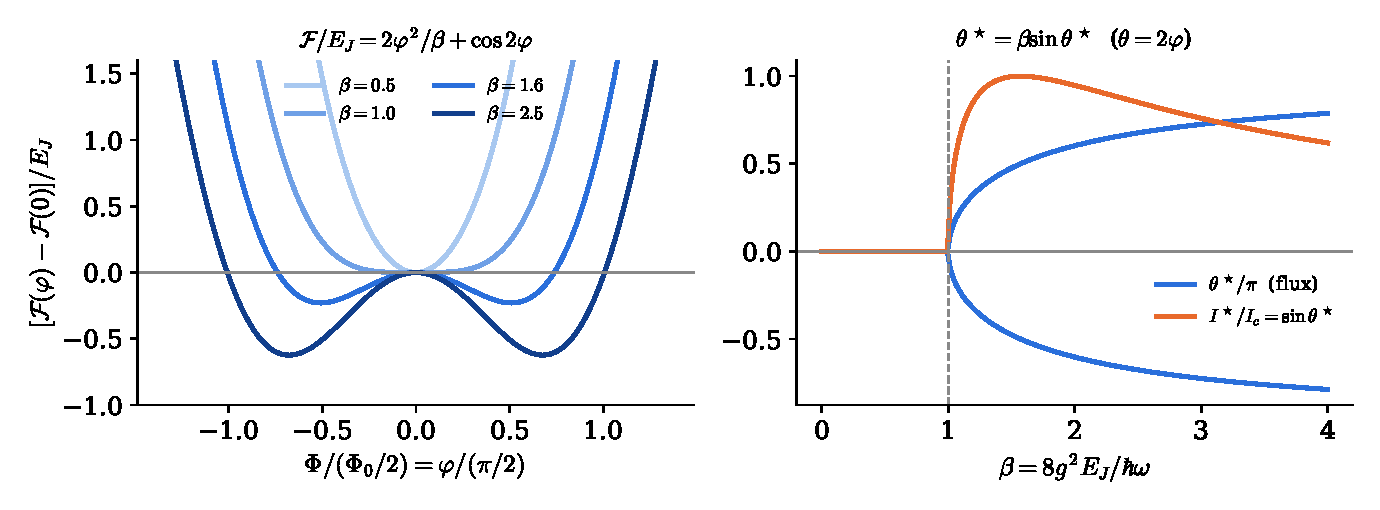
\includegraphics[width=0.92\textwidth]{landau.pdf}
  \begin{columns}[T]
    \column{0.5\textwidth}
    \small $\mathcal F'(X)=0$ with $\theta=2gX$:\quad
    $\dfrac{\hw}{2g}\,\varphi=2gE_J\sin2\varphi\ \Rightarrow\ \boxed{\theta^\star=\beta\sin\theta^\star}$
    \column{0.5\textwidth}
    \small $I^\star=I_c\sin\theta^\star$. Large $\beta$: $\theta^\star\to\pi$ (flux $\to\Phi_0/2$) and
    $I^\star\simeq\pi I_c/\beta\propto\hw/g^2$ \emph{decreases}.
  \end{columns}
\end{frame}

% ------------------------------------------------------------------
\begin{frame}{Below threshold: the soft mode}
  \begin{columns}[c]
    \column{0.5\textwidth}
    Expand to second order around $X=0$ ($\beta<1$):
    \[
      H_{\rm BO}\simeq\frac{\hw}{4}\Big(P^2+(1-\beta)X^2\Big)
    \]
    \begin{itemize}\small
      \item Excitation gap: $\boxed{\hw\sqrt{1-\beta}}$ \ (mode softening).
      \item Flux fluctuations grow: $\langle X^2\rangle=(1-\beta)^{-1/2}$.
      \item Photons in the ground state:
        $\langle n\rangle=\tfrac14\big[(1-\beta)^{-\frac12}+(1-\beta)^{\frac12}\big]-\tfrac12$.
    \end{itemize}
    \begin{calcbox}[title={Check against full DMRG ($U=2\Delta$)}]
      \footnotesize $\beta=0.5$: gap $\sqrt{0.5}=0.707$ vs DMRG $0.70$.\ \ $\beta=1$: DMRG $0.24$ (quartic regime).
      $\beta=1.5$: DMRG resolves $\delta=2.65\times10^{-4}\hw$ directly.
    \end{calcbox}
    \column{0.5\textwidth}
    \centering
    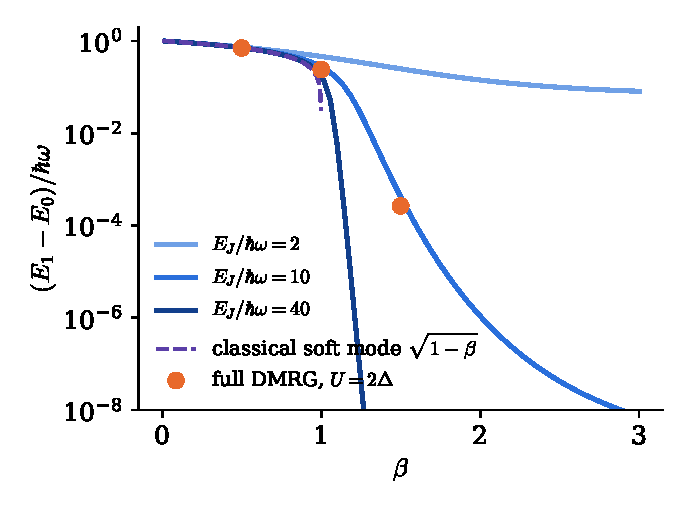
\includegraphics[width=0.93\textwidth]{soft_mode.pdf}
    \par\small At $\beta\to1$ the quadratic theory fails; above, the gap becomes the \alert{tunnel splitting}
    and collapses exponentially.
  \end{columns}
\end{frame}

% ------------------------------------------------------------------
\begin{frame}{Quantum fluctuations oppose the transition}
  \centering
  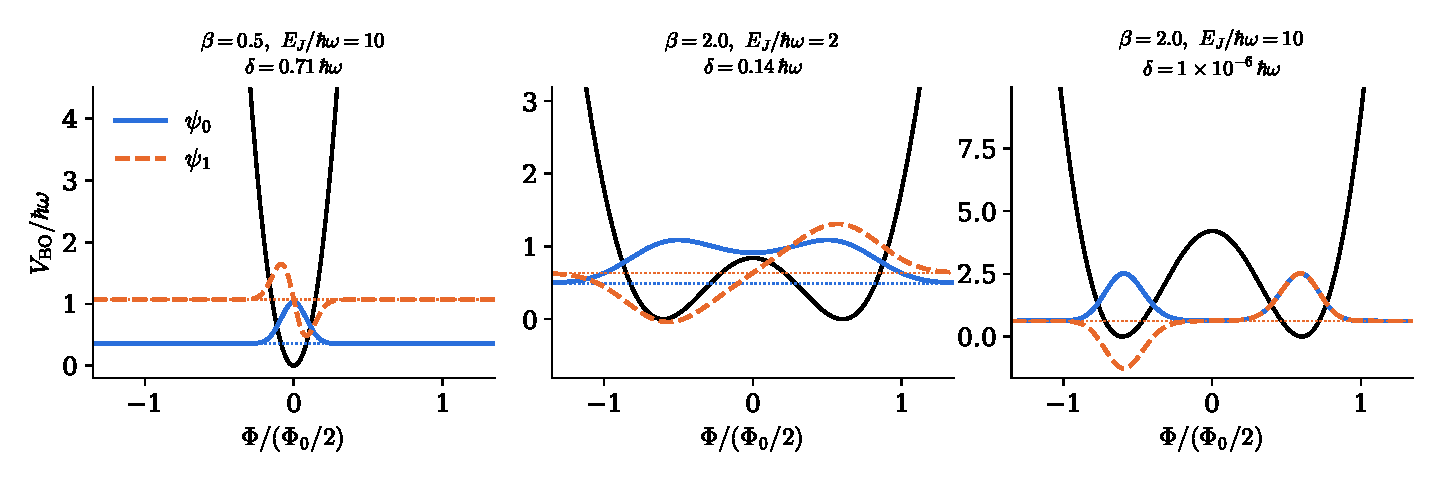
\includegraphics[width=0.93\textwidth]{quantum_well.pdf}
  \vspace{-1mm}
  \begin{columns}[T]
    \column{0.5\textwidth}
    \small Exact eigenstates of $H_{\rm BO}$ (pure $\pi$ junction). For $\beta>1$:
    $\psi_{0,1}\simeq(|\ccw\rangle\pm|\cw\rangle)/\sqrt2$ --- \alert{cat states} of macroscopic current, split by $\delta$.
    \column{0.5\textwidth}
    \small Zero-point fluctuations \emph{restore} the symmetry \cite{Bamba--Imoto 2017}: if the barrier is below $\sim\hw$
    (middle) there is no current-carrying state at all.
  \end{columns}
\end{frame}

% ------------------------------------------------------------------
\begin{frame}{How small is $\delta$? An instanton estimate}
  \begin{columns}[T]
    \column{0.55\textwidth}
    Particle of mass $M=\hbar^2/8E_C$ in $U(\theta)=E_J\,u(\theta)$,
    $u=\frac{\theta^2}{2\beta}+\cos\theta$. WKB:
    \[
      \delta\sim\hw\,e^{-S},\quad
      S=\int_{-\theta^\star}^{\theta^\star}\!d\theta\,\sqrt{\frac{U-U_{\min}}{4E_C}}
    \]
    \begin{calcbox}[title={Scaling}]
      \small $\dfrac{E_J}{4E_C}=\dfrac{E_J}{4g^2\hw}=\dfrac{2}{\beta}\Big(\dfrac{E_J}{\hw}\Big)^2$
      $\ \Rightarrow\ \boxed{S=\dfrac{E_J}{\hw}\,s(\beta)}$\\[1mm]
      $s(\beta)=\sqrt{2/\beta}\int\!d\theta\,\sqrt{u-u_{\min}}$.\\
      Near threshold ($\epsilon=1-1/\beta$): $u\simeq1-\frac{\epsilon}{2}\theta^2+\frac{\theta^4}{24}$,
      minima at $\theta^2=6\epsilon$, depth $\frac32\epsilon^2$ $\Rightarrow s\propto(\beta-1)^{3/2}$.
    \end{calcbox}
    \column{0.43\textwidth}
    \begin{keybox}[title={Sharp transition only in a scaling limit}]
      \small $E_J/\hw\to\infty$ at fixed $\beta$:
      \[
        \frac{E_C}{E_J}=\frac{\beta}{8}\Big(\frac{\hw}{E_J}\Big)^2\to0 ,
      \]
      flux becomes classical, $\delta\to0$, pitchfork with mean-field exponents.
    \end{keybox}
    \small Cf.\ quantum Rabi model: QPT only for $\Omega/\omega\to\infty$ \cite{Hwang--Puebla--Plenio 2015}.
    Finite $E_J/\hw$: a crossover; $\delta$ = macroscopic quantum tunnelling of the current.
  \end{columns}
\end{frame}

% ------------------------------------------------------------------
\begin{frame}{Limit 2 ($\hw\gg E_A$): Lang--Firsov, the Franck--Condon reduction}
  \begin{columns}[T]
    \column{0.55\textwidth}
    When the mode is fast, it stays in its vacuum and the electrons see the \emph{vacuum average} of the
    Peierls factor. Lang--Firsov transformation \cite{Lang--Firsov 1963}:
    \[
      D=e^{ig(a+a^\dagger)}=e^{-g^2/2}\,e^{iga^\dagger}e^{iga}\quad\Rightarrow\quad\langle0|D|0\rangle=e^{-g^2/2}
    \]
    \begin{keybox}
      \centering$\displaystyle H\to\Hring\ \text{with}\ t_J\to t_J\,e^{-g^2/2}\ \text{on the dressed bond},\ +O(t_J^2/\hw)$
    \end{keybox}
    \small The zero-point flux reduces the level width of the dot by the Franck--Condon factor $e^{-g^2}$ --
    on \emph{one} of its two bonds.
    \column{0.43\textwidth}
    \begin{calcbox}[title={Why this matters for $0$ vs $\pi$}]
      \small The singlet is bound by $\Gamma$ (YSR/Kondo screening); the doublet is not.
      Reducing $\Gamma$ favours the \alert{doublet}: the boundary $U_c$ moves \emph{down}.
    \end{calcbox}
    \begin{calcbox}[title={Adiabatic mechanism, for comparison}]
      \small Zero-point motion samples $E_s(gX)$ around $\varphi=0$:
      $\delta E_s\simeq\tfrac12g^2E''_s(0)\langle X^2\rangle$. Singlet curves \emph{up} ($E''_{\rm even}(0)=+0.20\Delta$) and loses;
      doublet curves down and gains, then relaxes its flux towards $\Phi_0/2$. Also moves $U_c$ \emph{down}.
    \end{calcbox}
    \small Neither limit is assumed in the DMRG; both are compared with it.
  \end{columns}
\end{frame}

% ==================================================================
\section{Methods}

\begin{frame}{Three levels of description}
  \centering
  \small
  \renewcommand{\arraystretch}{1.25}
  \begin{tabular}{@{}>{\raggedright}m{0.17\textwidth}>{\raggedright}m{0.42\textwidth}>{\raggedright}m{0.12\textwidth}m{0.18\textwidth}@{}}
    \toprule
    & ansatz & photon & cost \\ \midrule
    \textbf{Mean field} (MF) & $|\psi_{\rm el}\rangle\otimes|\chi_{\rm ph}\rangle$, self-consistent; HF--BdG electrons
      \cite{Varrica 2026; Andolina 2020} & product state & trivial \\
    \textbf{Circuit model} & $H^{(s)}_{\rm BO}$ with the DMRG $E_s(\varphi)$ at $g=0$ (fermions integrated out) &
      \alert{exact} & 1D Schr\"odinger \\
    \textbf{Lang--Firsov} & $\Hring$ with $t_Je^{-g^2/2}$ & vacuum & BdG/DMRG of the ring \\
    \textbf{Full DMRG} & MPS on electrons $\otimes$ photon, no approximation & \alert{exact} & 427 points $\approx$ 20 CPU\,h \\ \bottomrule
  \end{tabular}
  \vspace{3mm}
  \begin{keybox}
    \small Full DMRG is the result \emph{and} the referee: the circuit model and Lang--Firsov are its two limits,
    mean field is the ansatz used in the literature for this circuit.
  \end{keybox}
\end{frame}

% ------------------------------------------------------------------
\begin{frame}{Mean field and its hidden assumptions}
  \begin{columns}[T]
    \column{0.52\textwidth}
    \small Product state $\Rightarrow$ two coupled problems:
    \begin{align*}
      \text{el.:}&\ \Hring\ \text{(HF--BdG) with}\ t_J\to t_J\,\alpha,\quad \alpha=\langle\chi|D|\chi\rangle\\
      \text{ph.:}&\ \hw a^\dagger a-\big(\eta\,D+\text{h.c.}\big),\quad
      \eta=t_Je^{i\pcl}\textstyle\sum_\sigma\langle c^\dagger_{1\sigma}c_{0\sigma}\rangle\\
      E_{\rm MF}&=E_{\rm el}+E_{\rm ph}+2\,\mathrm{Re}(\eta\alpha)\ \ \text{(double counting)}
    \end{align*}
    For a coherent state $|X_0\rangle$: \ $\alpha=e^{igX_0}\,\alert{e^{-g^2/2}}$.
    \column{0.46\textwidth}
    \begin{warnbox}[title={(i) Not gauge covariant}]
      \footnotesize The junction bond is shrunk by $e^{-g^2/2}$ and loses phase-\emph{independent} kinetic energy,
      which the exact state recovers by following the flux.
    \end{warnbox}
    \begin{warnbox}[title={(ii) Self-trapping}]
      \footnotesize A product state must pick one well: it breaks the $\mathbb Z_2$ by construction, even when the
      barrier is below the zero-point energy.
    \end{warnbox}
    \begin{warnbox}[title={(iii) Static moment}]
      \footnotesize Hartree--Fock replaces the Kramers doublet by a polarized moment: $U_c^{\rm MF}=0.82\Delta$ for every $g$.
    \end{warnbox}
  \end{columns}
\end{frame}

% ------------------------------------------------------------------
\begin{frame}{Full DMRG for electrons + photon, and why the protocol matters}
  \begin{columns}[c]
    \column{0.5\textwidth}
    \centering
    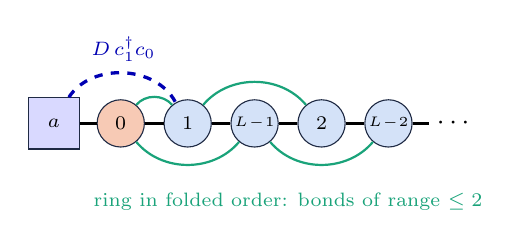
\begin{tikzpicture}[x=0.85cm,
        site/.style={circle,draw=ink,fill=accent!20,minimum size=6mm,inner sep=0pt,font=\scriptsize},
        dot/.style={circle,draw=ink,fill=warm!35,minimum size=6mm,inner sep=0pt,font=\scriptsize},
        bos/.style={rectangle,draw=ink,fill=blue!15,minimum size=6.5mm,inner sep=0pt,font=\scriptsize}]
      \node[bos] (b) at (0,0) {$a$};
      \node[dot] (s0) at (1,0) {$0$};
      \node[site] (s1) at (2,0) {$1$};
      \node[site] (sL) at (3,0) {\tiny$L\!-\!1$};
      \node[site] (s2) at (4,0) {$2$};
      \node[site] (sL2) at (5,0) {\tiny$L\!-\!2$};
      \node at (6,0) {$\cdots$};
      \draw[thick] (b)--(s0)--(s1)--(sL)--(s2)--(sL2)--(5.6,0);
      \draw[good,thick,bend left=50] (s0) to (s1);
      \draw[good,thick,bend left=50] (s1) to (s2);
      \draw[good,thick,bend right=50] (s0) to (sL);
      \draw[good,thick,bend right=50] (sL) to (sL2);
      \draw[blue!70!black,very thick,dashed,bend left=60] (b) to node[above,font=\scriptsize] {$D\,c^\dagger_1c_0$} (s1);
      \node[font=\scriptsize,good] at (3.5,-1.0) {ring in folded order: bonds of range $\le2$};
    \end{tikzpicture}
    \begin{itemize}\footnotesize
      \item TeNPy, two-site DMRG; photon = bosonic site, Fock cutoff $20$--$62$; parity and $S^z$ conserved;
            $\chi=200$--$400$ (truncation error $<2\times10^{-8}$).
      \item Benchmarks: BdG at $g=0$ ($10^{-14}$); ED of a 4-site ring + photon with sum rule ($10^{-7}$).
    \end{itemize}
    \column{0.5\textwidth}
    \begin{warnbox}[title={The energy is not the criterion}]
      \footnotesize The two current states differ only by $\delta$ and the seed, $2I^\star\pcl\sim10^{-5}\Delta$: DMRG
      drifts towards the polarized state over tens of sweeps and can stop \emph{under-polarized} within $10^{-6}\Delta$
      of the ground state. (An earlier warm-start scan had this problem; the sum rule exposed it.)
    \end{warnbox}
    \begin{keybox}[title={Protocol for every seeded point}]
      \footnotesize Two starts: (A) warm start from the vacuum side; (C) coherent state at the classical flux, annealed
      through seeds $10^{-2}\to3\cdot10^{-3}\to10^{-3}$. Keep the lower energy if they differ by $>3\times10^{-7}\Delta$,
      else report a \emph{bracket} (47/427, all inside crossovers). Accept only if the sum rule holds to $10^{-3}I_c$.
      Seed $10^{-4}$: current unchanged above threshold, $\times0.09$ below.
    \end{keybox}
  \end{columns}
\end{frame}

% ==================================================================
\section{Results}

\begin{frame}{The junction alone ($g=0$): three crossings, not one}
  \centering
  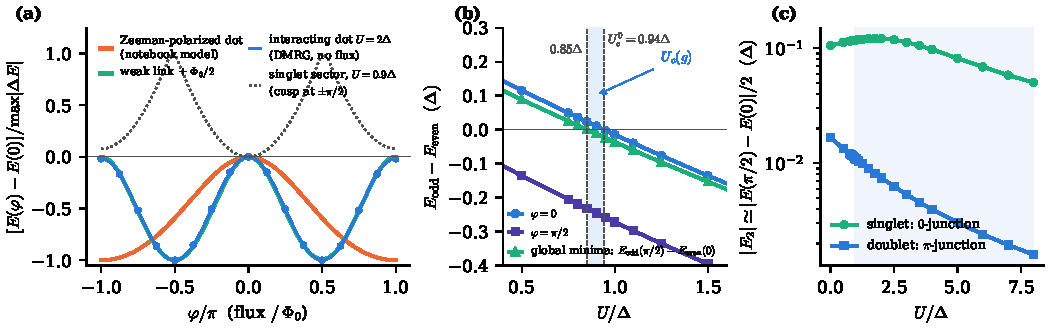
\includegraphics[width=0.95\textwidth]{fig_junctions.pdf}
  \begin{columns}[T]
    \column{0.34\textwidth}
    \small (a) The $U=2\Delta$ doublet at \emph{zero} flux $\equiv$ weak link + $\Phi_0/2$: $E_2=7.39\times10^{-3}\Delta$,
    $|E_1|/E_2=2\%$, $|E_4|/E_2<1\%$. Dotted: the \alert{singlet surface has a cusp} at $\pm\pi/2$ (two even states cross).
    \column{0.33\textwidth}
    \small (b) $U_c^0=0.94\Delta$: crossing at zero flux (the junction's own $0$--$\pi$ transition).
    $0.85\Delta$: crossing of the \emph{global minima} $E_{\rm odd}(\pi/2)=E_{\rm even}(0)$. Between: the $\pi'$ window
    \cite{Vecino 2003; Karrasch 2008}.
    \column{0.33\textwidth}
    \small (c) $E_2\propto U^{-1.3}$, approaching the $1/U$ of cotunnelling.
    \par\vspace{1mm}\textbf{In the $\pi'$ window a loop with a free flux switches to the doublet by letting
    $\Phi_0/2$ in.} The mode does exactly that.
  \end{columns}
\end{frame}

% ------------------------------------------------------------------
\begin{frame}{Result 1: the zero-point flux switches the loop from $0$ to $\pi$}
  \centering
  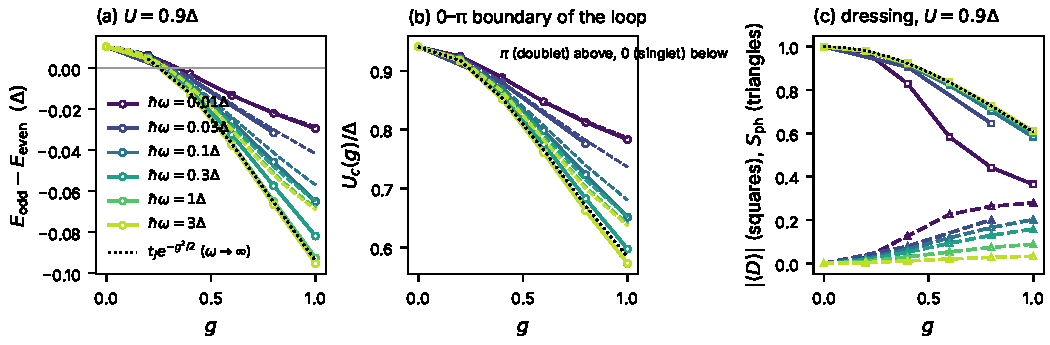
\includegraphics[width=0.95\textwidth]{fig_cavity_0pi.pdf}
  \begin{columns}[T]
    \column{0.34\textwidth}
    \small (a) $U=0.9\Delta$, $\hw=0.1\Delta$: $E_{\rm odd}-E_{\rm even}$ falls from $+0.010\Delta$ ($g=0$) to
    $-0.008\Delta$ ($g=0.4$) and $-0.065\Delta$ ($g=1$). Switch at $g\simeq0.28$, $Z\simeq0.6\,$k$\Omega$ --
    \alert{no seed, no flux, only the vacuum}.
    \column{0.33\textwidth}
    \small (b) $U_c(g,\omega)$ from $E_{\rm odd}=E_{\rm even}$, both sectors by full DMRG: $0.94\to0.83\Delta$ at $g=0.5$;
    $0.65$, $0.60$, $0.57\Delta$ at $g=1$ for $\hw=0.1$, $0.3$, $1\Delta$ ($30$--$40\%$).
    \column{0.33\textwidth}
    \small (c) Dressing: $|\langle D\rangle|$ follows $e^{-g^2/2}$ for $\hw\gtrsim0.3\Delta$ (vacuum only squeezed),
    falls faster in the adiabatic regime (mode displaced towards the $\pi$ well); entanglement $S_{\rm ph}$ largest
    there ($0.26$).
  \end{columns}
\end{frame}

% ------------------------------------------------------------------
\begin{frame}{Result 1, mechanism: from the adiabatic flux average to Franck--Condon}
  \begin{columns}[T]
    \column{0.55\textwidth}
    \centering\small $U_c(g,\omega)/\Delta$ of the loop (full DMRG), $U_c^0=0.941$:\\[1mm]
    \scriptsize
    \begin{tabular}{@{}lccccc@{}}
      \toprule
      $\hw/\Delta$ & $g=0.2$ & $0.4$ & $0.6$ & $0.8$ & $1.0$\\ \midrule
      0.01 & 0.925 & 0.889 & 0.848 & 0.813 & 0.783\\
      0.1 & 0.921 & 0.868 & 0.798 & 0.724 & 0.652\\
      0.3 & 0.919 & 0.859 & 0.775 & 0.683 & 0.597\\
      1.0 & 0.918 & 0.853 & 0.762 & 0.663 & 0.573\\
      3.0 & 0.917 & 0.852 & 0.761 & 0.662 & 0.573\\ \midrule
      circuit model ($\hw=0.01$) & 0.925 & 0.889 & 0.849 & 0.815 & 0.787\\
      Lang--Firsov ($\omega\to\infty$) & 0.918 & 0.854 & 0.765 & 0.670 & 0.584\\ \bottomrule
    \end{tabular}
    \column{0.43\textwidth}
    \begin{itemize}\footnotesize
      \item $\hw\ll E_A$: exact = circuit model to $2\times10^{-3}\Delta$ (curvatures + relaxation towards $\Phi_0/2$;
            bounded by the condensation energy of the $\pi$ well).
      \item $\hw\gtrsim\Delta$: exact = Lang--Firsov to $10^{-2}\Delta$, saturated by $\hw\simeq\Delta$
            (bounded by $\Gamma$; corrections $O(t_J^2/\hw)<0.01\Delta$).
      \item Not an artefact of the one-bond vertex: the neglected $O(\hw g^2/E_A)$ vanish at $\hw=0.01\Delta$, where
            the shift is already half of that at $0.3\Delta$.
      \item Not mean field: HF puts the boundary at $0.82\Delta$ for \emph{every} $g$.
    \end{itemize}
    \begin{keybox}
      \footnotesize Prediction: a dot gate-tuned near its parity boundary, in a loop with a $Z\gtrsim1\,$k$\Omega$
      superinductor, is driven into the $\pi$ phase \emph{by the impedance alone} -- the resonator-frequency jump of
      \cite{Bargerbos 2022; Pita-Vidal 2023}.
    \end{keybox}
  \end{columns}
\end{frame}

% ------------------------------------------------------------------
\begin{frame}{Result 2 (central): the $(U,g)$ phase diagram from full DMRG}
  \centering
  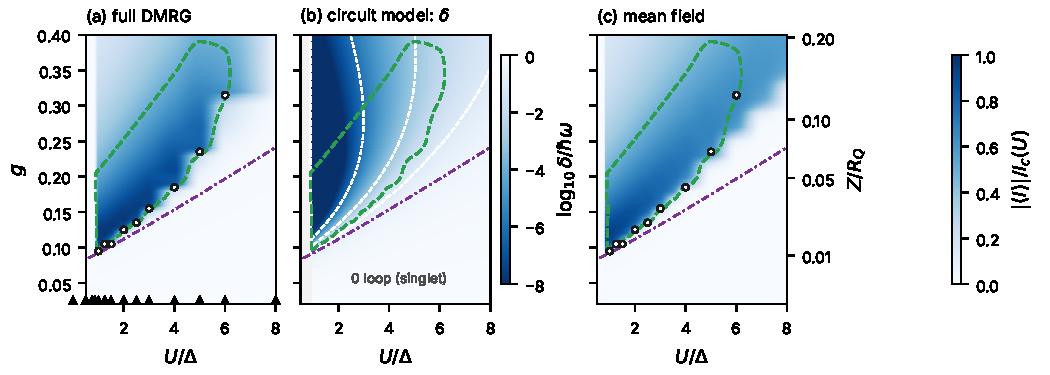
\includegraphics[width=0.88\textwidth]{fig_phase_main.pdf}
  \vspace{-1mm}
  \begin{columns}[T]
    \column{0.34\textwidth}
    \footnotesize (a) \textbf{Full DMRG}, $427$ ground states: $g=0.02$--$0.40$, $14$ values of $U$ (triangles), both sectors
    for $U\le\Delta$, seed $10^{-3}$, $\chi=300$. Colour: $|\langle I\rangle|/I_c(U)$; circles: $0.5I_c$.
    \column{0.33\textwidth}
    \footnotesize (b) Seed-free order parameter of the circuit model: tunnel splitting $\delta(U,g)$ (white:
    $10^{-1},10^{-3},10^{-6}\hw$); grey: singlet $0$ loop. Same boundary as $\delta=0.1\hw$.
    \column{0.33\textwidth}
    \footnotesize (c) Mean field. Green dashed: $0.5I_c$ contour of the circuit model; purple: classical $\beta=1$.
    Right axis: $Z/R_Q=4g^2/\pi$ ($g=0.4$ is $Z=1.3\,$k$\Omega$).
  \end{columns}
  \par\footnotesize\hl{$\hw=7.39\times10^{-4}\Delta$ is chosen so that $E_J/\hw$ runs from $15$ ($U\simeq\Delta$) to $2$ ($U=8\Delta$):
  one picture holds both the sharp transition and its quantum smearing.}
\end{frame}

% ------------------------------------------------------------------
\begin{frame}{Reading the phase diagram: three regions}
  \begin{columns}[T]
    \column{0.5\textwidth}
    \begin{exampleblock}{(i) $U<U_c(g)$: the $0$ loop}
      \footnotesize Singlet ground state, diamagnetic, mode \emph{stiffened} ($\omega'$ up to $9.4\omega$), squeezed vacuum,
      current $<10^{-2}I_c$ and linear in the seed. Boundary moves $0.94\to0.85\Delta$ at $g=0.4$ = the global-minimum
      crossing: the adiabatic end of Result 1.
    \end{exampleblock}
    \begin{alertblock}{(ii) $U>U_c$, $g>g_c(U)$: the condensate}
      \footnotesize $U=2\Delta$: $\langle n\rangle$ $0.5\to7.3$ for $g=0.11\to0.14$, current $0.96I_c$, then
      $I\simeq\hw\varphi^\star/2g^2$ (flux saturates at $\Phi_0/2$, inductance grows).
      $g_c=0.10,0.13,0.19,0.24,0.32$ at $U/\Delta=1,2,4,5,6$: \alert{above $\beta=1$} by $\Delta g=0.02,0.04,0.12$
      at $E_J/\hw=10,5,3.2$; crossover widens to $\Delta g=0.08$; $I_{\max}$ falls $0.97\to0.61\,I_c$.
    \end{alertblock}
    \column{0.5\textwidth}
    \begin{block}{(iii) $U=8\Delta$ ($E_J/\hw=2.1$): no order}
      \footnotesize $\beta$ reaches $2.7$ but the ground state is the cat with $\delta\simeq\hw$; current $\le0.04I_c$,
      $\propto$ seed.
    \end{block}
    \begin{calcbox}[title={Full DMRG vs circuit model, above threshold}]
      \footnotesize $0.2\%$ of $I_c$ on average ($2.4\%$ worst), $0.1$ in photon number, $10^{-5}\Delta$ in energy:
      at $\hw/E_A\sim10^{-3}$ the fluxonium with the microscopic $E_s(\varphi)$ \emph{is} the exact circuit model.
    \end{calcbox}
    \begin{warnbox}[title={Mean field}]
      \footnotesize $g_c$ right to one grid step for $U\le5\Delta$, current $10$--$20\%$ low, $\langle n\rangle$ high at large $g$
      ($5.2$ vs $3.7$); orders $U=7$--$8\Delta$ with $0.6I_c$ (absent); orders $U=0.85\Delta$ with $0.95I_c$ where the exact
      state is the singlet $0$ loop.
    \end{warnbox}
  \end{columns}
\end{frame}

% ------------------------------------------------------------------
\begin{frame}{Cuts through the diagram}
  \centering
  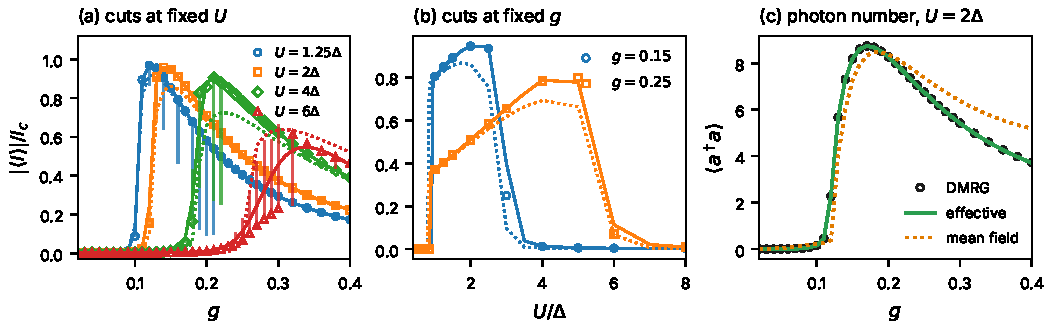
\includegraphics[width=0.95\textwidth]{fig_phase_slices.pdf}
  \begin{columns}[T]
    \column{0.5\textwidth}
    \small (a),(b) Symbols: full DMRG (bars: brackets between the two starts, all inside crossovers); solid:
    circuit model; dotted: mean field. The sharp step at $U=1.25,2\Delta$ becomes a broad crossover at $U=6\Delta$.
    \column{0.5\textwidth}
    \small (c) Photon number at $U=2\Delta$: the condensate of $\simeq7$--$9$ photons is a \emph{static flux}
    ($\langle n\rangle\simeq\langle X\rangle^2/4$), not radiation. Mean field overshoots at large $g$.
  \end{columns}
\end{frame}

% ------------------------------------------------------------------
\begin{frame}{Result 3: the cat state and macroscopic tunnelling of a current}
  \centering
  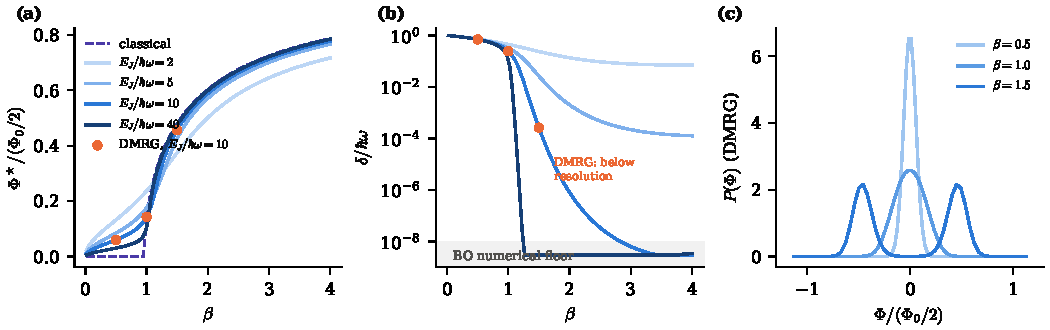
\includegraphics[width=0.9\textwidth]{fig_udot_cavity.pdf}
  \begin{columns}[T]
    \column{0.34\textwidth}
    \small $U=2\Delta$, $E_J/\hw=10$, no flux, no seed: $H$ real $\Rightarrow\langle I\rangle=0$ in every eigenstate.
    (a) The flux projected on the lowest doublet has eigenvalues $\pm\Phi^\star$
    ($0.59\,\Phi_0/2$ at $\beta=2$; DMRG = circuit model to $0.2\%$).
    \column{0.33\textwidth}
    \small (b) $\delta/\hw=0.70$, $0.24$, $2.65\times10^{-4}$ at $\beta=0.5,1,1.5$; the last one
    \alert{resolved directly by DMRG} ($\chi=300$ vs $400$: $2.66$ vs $2.65\times10^{-4}$): tunnelling of a
    seven-photon condensate, $\delta=2\times10^{-7}\Delta$. Beyond: circuit model, $8\times10^{-7}$, $6.5\times10^{-9}$ at $\beta=2,3$.
    \column{0.33\textwidth}
    \small (c) The DMRG ground state \emph{is} the cat: $|\langle\Phi\rangle|<10^{-3}\Phi^\star$, bimodal $P(\Phi)$;
    a run started from the polarized state relaxes to it ($10^{-10}\Delta$).
    Manifold: $\{\uparrow,\downarrow\}\otimes\{\cw,\ccw\}$, split only by $\delta$.
  \end{columns}
\end{frame}

% ------------------------------------------------------------------
\begin{frame}{Where the product state fails: a cautionary tale ($E_J\simeq\hw$)}
  \begin{columns}[c]
    \column{0.4\textwidth}
    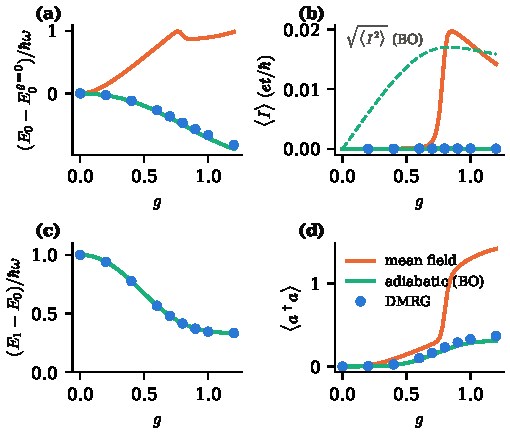
\includegraphics[width=\textwidth]{fig_notebook_model.pdf}
  \column{0.58\textwidth}
    \footnotesize Short ring ($L=11$), Zeeman-polarized dot, $\hw=0.02$: the ansatz of \cite{Varrica 2026; Andolina 2020}
    (and of our own first treatment).
    \begin{itemize}\footnotesize
      \item MF: current-carrying phase for $g\gtrsim0.75$, $\langle n\rangle\simeq1.4$.
      \item DMRG: \alert{no current} (linear response $7\times10^{-5}$), energy $1.8\hw$ \emph{below} MF, gap stays
            $0.33\hw$, $\langle n\rangle\simeq0.36$. Circuit model = DMRG.
    \end{itemize}
    \begin{warnbox}[title={Three reasons}]
      \footnotesize (1) product state not gauge covariant; (2) $E_J\simeq\hw$: double well shallower than the zero-point
      energy, $P(X)$ unimodal; (3) $L\lesssim\xi$: $E_1\gg E_2$, the instability would be of the \emph{normal} $h/e$ current.
    \end{warnbox}
    \footnotesize Same model at $\hw=0.002$: it does order, $g_c=0.21$ (MF: $0.30$). \alert{The control parameter is $E_J/\hw$.}
  \end{columns}
\end{frame}

% ------------------------------------------------------------------
\begin{frame}{With spin--orbit coupling: spin-locked currents instead of a cat}
  \centering
  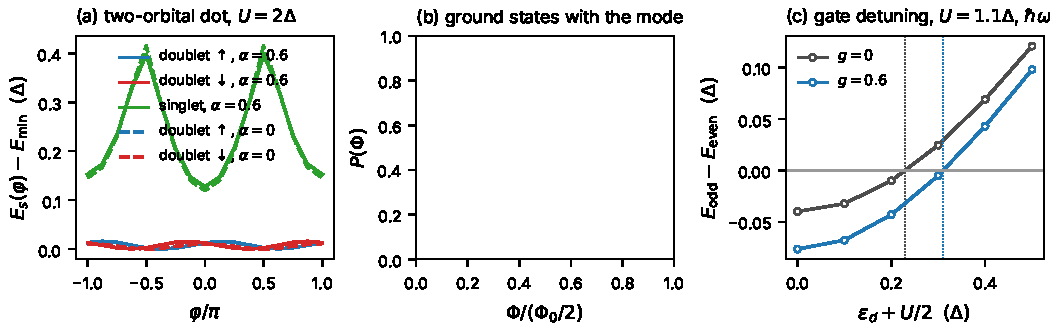
\includegraphics[width=0.9\textwidth]{fig_so.pdf}
  \begin{columns}[T]
    \column{0.34\textwidth}
    \footnotesize Two-orbital dot, spin-dependent phase $e^{i\alpha\sigma^z}$ on one of two interfering paths
    ($\alpha=0.6$; in one channel it gauges away). (a) Doublet surfaces
    $E_\sigma=E_0+E_2\cos(2\varphi-2\sigma\varphi_{\rm so})$, $\varphi_{\rm so}=0.42$ ($24^\circ$).
    \column{0.33\textwidth}
    \footnotesize (b) With the mode ($\beta=2$): the two wells of a given spin are split by $2E_2\sin2\varphi_{\rm so}$;
    $\uparrow$ sits at $-\Phi^\star$, $\downarrow$ at $+\Phi^\star$ ($\mp0.51\,\Phi_0/2$, $6.5$ photons). The manifold is
    one Kramers pair $\{|{\uparrow}{\ccw}\rangle,|{\downarrow}{\cw}\rangle\}$: the inductively protected spin qubit of
    \cite{del Olmo 2026}.
    \column{0.33\textwidth}
    \footnotesize (c) Gate: at $U=1.1\Delta$, $\hw=0.1\Delta$ the doublet window widens from $0.229$ to $0.310\Delta$ at $g=0.6$
    ($35\%$; $29\,\mu$eV in Al, $0.1$--$0.3$\,mV of gate). The flux-driven switch survives: $U_c^0=1.36\to1.15\Delta$.
  \end{columns}
\end{frame}

% ==================================================================
\section{Where to look}

\begin{frame}{Physical units: what is easy and what is hard}
  \begin{columns}[T]
    \column{0.5\textwidth}
    \begin{exampleblock}{Flux-driven $0$--$\pi$ switch: easy}
      \footnotesize $\hw=0.03$--$0.3\Delta$, $g=0.3$--$0.6$. Al ($\Delta=180\,\mu$eV): a $1$--$13$\,GHz mode sharing its
      inductance with the loop, $Z=4R_Qg^2/\pi=0.7$--$3\,$k$\Omega$ (granular Al, junction arrays
      \cite{Manucharyan 2009; Gr\"unhaupt 2019}), dot gate-tuned to $\sim0.1\Delta$ of its parity boundary
      \cite{Bargerbos 2022; Pita-Vidal 2023}. Readout: resonator-frequency jump; signature: driven by the impedance
      (superinductor length) at fixed gate.
    \end{exampleblock}
    \begin{alertblock}{Condensate and cat: hard}
      \footnotesize Need $E_J/\hw\gtrsim5$ and $\hw>k_BT$. The $U=2\Delta$, $\Gamma=\Delta/2$ junction has $E_J/h=0.3$\,GHz,
      $I_c=0.65$\,nA in Al $\Rightarrow$ $\hw=E_J/10=32$\,MHz: below the electron temperature.
    \end{alertblock}
    \column{0.5\textwidth}
    \tiny
    \begin{tabular}{@{}lccccc@{}}
      \toprule
      $U$, $\Gamma$, material & $E_J/h$ & $I_c$ & $E_J/10h$ & $E_J/10k_B$ & $L_{\beta=1}$\\ \midrule
      $2\Delta$, $\Delta/2$, Al & 0.32 GHz & 0.65 nA & 32 MHz & 1.5 mK & 510 nH\\
      $2\Delta$, $\Delta/2$, NbTiN & 2.1 GHz & 4.3 nA & 210 MHz & 10 mK & 76 nH\\
      $6\Delta$, $2\Delta$, Al & 1.5 GHz & 3.0 nA & 150 MHz & 7 mK & 110 nH\\
      $6\Delta$, $2\Delta$, NbTiN & 9.9 GHz & 20 nA & 0.99 GHz & 47 mK & 17 nH\\
      $6\Delta$, $2\Delta$, Nb & 11.5 GHz & 23 nA & 1.15 GHz & 55 mK & 14 nH\\ \bottomrule
    \end{tabular}
    \par\vspace{1mm}
    \begin{itemize}\small
      \item Strong junction ($\Gamma=2\Delta$, $U=6\Delta$, $E_J=0.034\Delta$) in NbTiN/Nb: $\simeq1$\,GHz mode, $L\simeq17$\,nH,
            $Z\simeq160\,\Omega$: a $\pi$-rf-SQUID at zero flux; full DMRG: $9.6$ photons, $0.94I_c$.
      \item nA dot + GHz superinductor: $E_J/\hw\lesssim3$, no current phase (the $U=8\Delta$ line) but the cat with
            $\delta\sim\hw$: dip of the $0\to1$ frequency, jump of $\langle0|\Phi|1\rangle$ in two-tone spectroscopy
            -- where MF predicts $0.6I_c$.
    \end{itemize}
  \end{columns}
\end{frame}

% ==================================================================
\section{Summary}

\begin{frame}{Take-home messages}
  \begin{enumerate}\small
    \item Dot electrons and quantized loop flux on the same footing: full DMRG, Peierls vertex to all orders,
          sum rule $\langle I\rangle=\langle\Phi\rangle/L$ as acceptance test.
    \item \alert{The vacuum of the mode controls the junction}: its zero-point flux moves the singlet--doublet boundary
          by $30$--$40\%$ at $g=1$ -- adiabatically through the curvatures of $E_s(\varphi)$, non-adiabatically through
          the Franck--Condon factor $t_J\to t_Je^{-g^2/2}$ -- at impedances $Z\sim1$--$3\,$k$\Omega$ that exist.
    \item \alert{Full-DMRG $(U,g)$ phase diagram}: the photon condensate is the screening instability $\beta>1$ of a
          $\pi$ loop; the exact ground state is the cat of the two current directions ($\delta$ resolved directly);
          zero-point motion pushes $g_c$ above $\beta=1$ and erases the phase for $E_J/\hw\lesssim2.5$. In the adiabatic
          regime the loop \emph{is} a fluxonium with the microscopic $E_s(\varphi)$.
    \item The product-state mean field \alert{orders where the exact solution does not}: at $E_J\lesssim3\hw$ and at
          $U\simeq U_c$ (static moment instead of the Kramers doublet).
    \item With spin--orbit the cat becomes a spin-locked persistent current (a protected spin qubit); the switch survives.
  \end{enumerate}
\end{frame}

% ------------------------------------------------------------------
\begin{frame}{Open questions}
  \begin{itemize}
    \item \textbf{Kondo regime} ($T_K\gg\Delta$): the junction returns to $0$ -- how does the switch look there?
    \item \textbf{Capacitive terms} of the displaced charge, $\hw g^2/E_A$: of order one at $\hw\gtrsim0.3\Delta$, $g\sim1$;
          a two-mode or transmission-line model would fix them.
    \item \textbf{Lead kinetic inductance}: with a rigid $\Delta$ all phase drops on the junction; a self-consistent BdG
          ring puts most of it in the leads (backup). How does it renormalize $\beta$ in a real loop?
    \item \textbf{Quasiparticle poisoning}: a parity flip is a $\pi\leftrightarrow0$ switch of the whole loop.
    \item \textbf{Dissipation and readout}: dispersive shift, $\langle0|\Phi|1\rangle$, finite $T$; multi-dot junctions.
  \end{itemize}
  \vfill
  \centering\Large Thank you!
\end{frame}

% ==================================================================
\appendix
\section*{Backup}

\begin{frame}{Backup: weak link biased by $\Phi_0/2$ ($L=14$, $E_J/\hw=10$)}
  \centering
  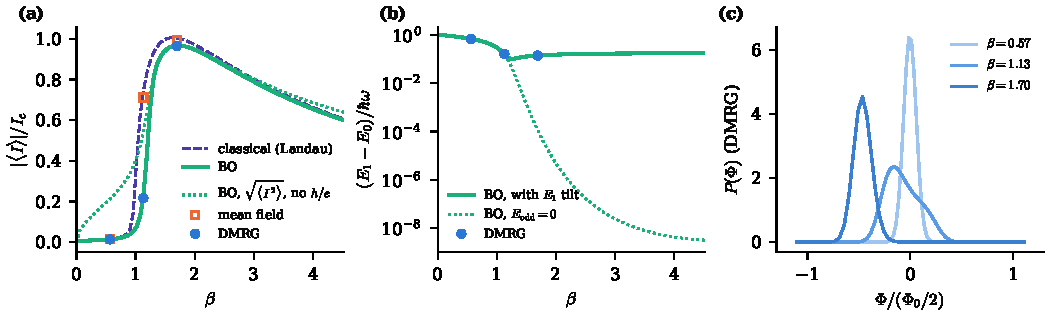
\includegraphics[width=0.92\textwidth]{fig_weaklink_halfflux.pdf}
  \begin{columns}[T]
    \column{0.34\textwidth}
    \small (a) Current rises at $\beta\simeq1.1$, saturates at $0.96I_c$. MF: $0.71$ vs $0.22I_c$ at $\beta=1.13$,
    $0.2$--$0.4\hw$ too high in energy. DMRG vs circuit model: $2\times10^{-3}\hw$, $2\%$ of $I_c$.
    \column{0.33\textwidth}
    \small (b) Splitting saturates: it is the \alert{tilt} $2|E_1|\sin\varphi^\star\approx0.2\hw$ of the residual
    $h/e$ harmonic, not tunnelling (without it $\delta<10^{-6}\hw$ at $\beta=2$).
    \column{0.33\textwidth}
    \small (c) $P(\Phi)$: a single displaced peak -- the direction is \emph{selected} by $E_1$. An intrinsic $\pi$
    junction removes the need for the $\Phi_0/2$ bias, not the sensitivity to a flux offset $\delta\Phi>\delta/2I^\star$.
  \end{columns}
\end{frame}

\begin{frame}{Backup: convergence of the full DMRG on the phase diagram}
  \centering
  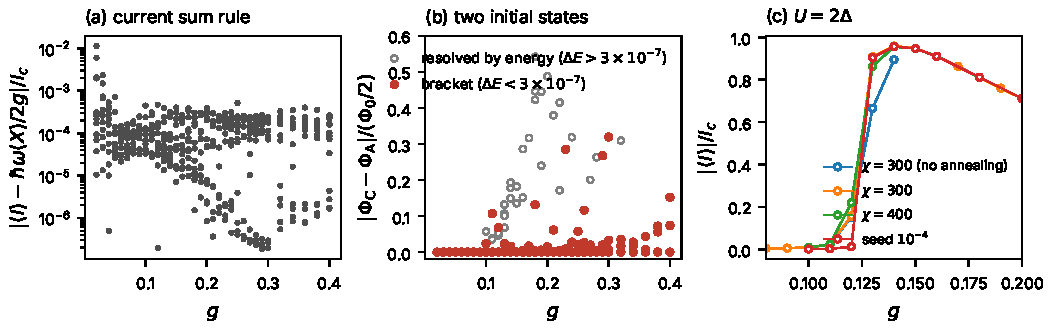
\includegraphics[width=0.95\textwidth]{fig_phase_convergence.pdf}
  \begin{columns}[T]
    \column{0.34\textwidth}
    \small (a) Sum-rule violation $|\langle I\rangle-\hw\langle X\rangle/2g|/I_c$ over the grid: median $10^{-4}$, all
    $<10^{-3}$ for $g\ge0.04$.
    \column{0.33\textwidth}
    \small (b) Flux difference between the two starts (vacuum side A, polarized side C): open = resolved by energy,
    filled = brackets ($47/427$).
    \column{0.33\textwidth}
    \small (c) $U=2\Delta$ near threshold: $\chi=300$ without/with annealing, $\chi=400$ (energies to $4\times10^{-8}\Delta$,
    current to $0.3\%$), seed $10^{-4}$.
  \end{columns}
\end{frame}

\begin{frame}{Backup: gauge covariance of the static phase; phase drop in self-consistent BdG}
  \begin{columns}[T]
    \column{0.52\textwidth}
    \small Non-interacting ring with a dot ($L=14$, $t_J=0.5$); BdG ground-state energy:\\[1mm]
    \tiny
    \begin{tabular}{@{}cccc@{}}
      \toprule
      $\varphi$ & one bond & uniform $\mathbf A$, covariant $\Delta_j$ & uniform $\mathbf A$, \alert{real} $\Delta$\\ \midrule
      $0$ & $-21.82094$ & $-21.82094$ & $-21.82094$\\
      $0.5$ & $-21.79739$ & $-21.79739$ & $-21.81251$\\
      $1.0$ & $-21.72957$ & $-21.72957$ & $-21.78725$\\
      $\pi/2$ & $-21.61009$ & $-21.61009$ & $-21.73791$\\ \bottomrule
    \end{tabular}
    \par\small First two agree to $10^{-10}$ (\texttt{tests/test\_gauge\_covariance.py}); a uniform $\mathbf A$ with a
    real $\Delta$ is a different model.
    \column{0.44\textwidth}
    \small Weak link ($t_J=0.5$, $L=14$) with $\Delta_j=-U_a\langle c_{j\downarrow}c_{j\uparrow}\rangle$ solved
    self-consistently (complex), $|\Delta|=1$:\\[1mm]
    \scriptsize
    \begin{tabular}{@{}ccc@{}}
      \toprule
      pair flux $2\varphi$ & junction drop & fraction\\ \midrule
      0.4 & 0.110 & 0.275\\
      0.8 & 0.221 & 0.277\\
      1.2 & 0.335 & 0.279\\ \bottomrule
    \end{tabular}
    \par\small Current conserved bond by bond; only $\approx28\%$ of the gauge-invariant phase drops on the junction in
    this short ring -- the leads act as a series kinetic inductance (\texttt{code/selfconsistent\_phase.py}).
  \end{columns}
\end{frame}

\begin{frame}{Backup: references}
  \scriptsize
  \begin{itemize}
    \item Bulaevskii, Kuzii, Sobyanin, JETP Lett.\ \textbf{25}, 290 (1977); Tsuei, Kirtley, RMP \textbf{72}, 969 (2000);
          Ryazanov \emph{et al.}, PRL \textbf{86}, 2427 (2001); Bauer \emph{et al.}, PRL \textbf{92}, 217001 (2004)
    \item Ioffe \emph{et al.}, Nature \textbf{398}, 679 (1999); Yamashita \emph{et al.}, PRL \textbf{95}, 097001 (2005);
          Kawabata \emph{et al.}, PRB \textbf{74}, 180502(R) (2006); Feofanov \emph{et al.}, Nat.\ Phys.\ \textbf{6}, 593 (2010)
    \item Nataf, Ciuti, Nat.\ Commun.\ \textbf{1}, 72 (2010); Bamba, Inomata, Nakamura, PRL \textbf{117}, 173601 (2016);
          Bamba, Imoto, PRA \textbf{96}, 053857 (2017); Andolina \emph{et al.}, PRB \textbf{100}, 121109(R) (2019); PRB \textbf{102}, 125137 (2020);
          Mercurio \emph{et al.}, Phys.\ Rev.\ Res.\ \textbf{6} (2024)
    \item Glazman, Matveev, JETP Lett.\ \textbf{49}, 659 (1989); Spivak, Kivelson, PRB \textbf{43}, 3740 (1991);
          Vecino \emph{et al.}, PRB \textbf{68}, 035105 (2003); Karrasch \emph{et al.}, PRB \textbf{77}, 024517 (2008);
          Meng, Florens, Simon, PRB \textbf{79}, 224521 (2009)
    \item van Dam \emph{et al.}, Nature \textbf{442}, 667 (2006); Cleuziou \emph{et al.}, Nat.\ Nano.\ \textbf{1}, 53 (2006);
          Delagrange \emph{et al.}, PRB \textbf{91}, 241401(R) (2015); Bargerbos \emph{et al.}, PRX Quantum \textbf{3}, 030311 (2022);
          Hays \emph{et al.}, Science \textbf{373}, 430 (2021); Pita-Vidal \emph{et al.}, Nat.\ Phys.\ \textbf{19}, 1110 (2023)
    \item Padurariu, Nazarov, PRB \textbf{81}, 144519 (2010); del Olmo \emph{et al.}, arXiv:2608.13530 (2026); Varrica \emph{et al.}, arXiv:2603.07256 (2026)
    \item Friedman \emph{et al.}, Nature \textbf{406}, 43 (2000); Manucharyan \emph{et al.}, Science \textbf{326}, 113 (2009);
          Gr\"unhaupt \emph{et al.}, Nat.\ Mater.\ \textbf{18}, 816 (2019); Hwang, Puebla, Plenio, PRL \textbf{115}, 180404 (2015)
    \item Li \emph{et al.}, PRB \textbf{101}, 205140 (2020); Dmytruk, Schir\`o, PRB \textbf{103}, 075131 (2021);
          Dmytruk, Trif, Simon, PRB \textbf{94}, 115423 (2016); Lang, Firsov, Sov.\ Phys.\ JETP \textbf{16}, 1301 (1963)
    \item Passetti \emph{et al.}, PRL \textbf{131}, 023601 (2023); Bacciconi \emph{et al.}, SciPost Phys.\ \textbf{15}, 113 (2023);
          Loss, Goldbart, PRB \textbf{43}, 13762 (1991); Hauschild, Pollmann, SciPost Phys.\ Lect.\ Notes 5 (2018)
  \end{itemize}
\end{frame}

\end{document}
